\documentclass[12pt,a4paper]{article}

% ================= PACOTES =================
\usepackage[utf8]{inputenc}
\usepackage[T1]{fontenc}
\usepackage[brazil]{babel}
\usepackage[top=3cm, bottom=2cm, left=3cm, right=2cm]{geometry}
\usepackage{graphicx}
\usepackage{listings}
\usepackage{xcolor}
\usepackage{caption}
\usepackage{float}
\usepackage{hyperref}
\usepackage{tabularx}
\newcolumntype{Y}{>{\centering\arraybackslash}X}
\usepackage{parskip}
\usepackage{titlesec}
\usepackage{fancyhdr}
\usepackage{booktabs}
\usepackage{enumitem}
\usepackage{indentfirst}
\usepackage{amsmath}
\usepackage{tcolorbox}

% ================= CONFIGURAÇÕES DE ESPAÇAMENTO =================
\setlength{\headheight}{15pt}
\setlength{\parindent}{1.25cm}
\setlength{\parskip}{6pt}

% ================= CORES E ESTILOS DE CÓDIGO =================
\definecolor{kw}{HTML}{00008B}
\definecolor{comm}{HTML}{228B22}
\definecolor{strcolor}{HTML}{8B0000}
\definecolor{bgcolor}{HTML}{F8F8F8}

\lstdefinestyle{sql}{
  language=SQL,
  basicstyle=\ttfamily\small,
  keywordstyle=\color{kw}\bfseries,
  commentstyle=\color{comm}\itshape,
  stringstyle=\color{strcolor},
  backgroundcolor=\color{bgcolor},
  breaklines=true,
  showstringspaces=false,
  aboveskip=8pt,
  belowskip=8pt,
  frame=single,
  rulecolor=\color{gray},
  morekeywords={OPENROWSET, BULK, FORMAT, HEADER_ROW, PARSER_VERSION,
                FIELDTERMINATOR, FIELDQUOTE, ROWTERMINATOR, COLLATE,
                JSON_VALUE, TOP, WITH, CAST, FLOAT}
}

\lstdefinestyle{json}{
  basicstyle=\ttfamily\small,
  backgroundcolor=\color{bgcolor},
  breaklines=true,
  showstringspaces=false,
  frame=single,
  rulecolor=\color{gray},
  aboveskip=8pt,
  belowskip=8pt
}

% ================= ESTILO DE TÍTULOS =================
\titleformat{\section}{\large\bfseries}{\thesection.}{0.5em}{}
\titleformat{\subsection}{\normalsize\bfseries}{\thesubsection.}{0.5em}{}
\titleformat{\subsubsection}{\normalsize\bfseries}{\thesubsubsection.}{0.5em}{}

% ================= CABEÇALHO E RODAPÉ =================
\pagestyle{fancy}
\fancyhf{}
\fancyhead[L]{\small PUCRS - Escola Politécnica}
\fancyhead[R]{\small Porto Alegre, \today}
\fancyfoot[R]{\thepage}
\renewcommand{\headrulewidth}{0.4pt}

% ================= LEGENDAS =================
\captionsetup{font=small, labelfont=bf, justification=centering, skip=4pt}
\renewcommand{\figurename}{Figura}
\renewcommand{\tablename}{Tabela}

\hypersetup{colorlinks=true, linkcolor=black, urlcolor=blue}

% Caixa de espaço reservado para imagens
\newcommand{\imagemPendente}[2]{%
  \begin{figure}[H]
    \centering
    \begin{tcolorbox}[width=#1, halign=center, valign=center, height=6cm,
      colback=gray!10, colframe=gray!50]
      \textit{[Imagem a inserir: #2]}
    \end{tcolorbox}
    \caption{#2}
  \end{figure}
}

\begin{document}

% ================= CAPA =================
\begin{titlepage}
  \centering
  \vspace*{1cm}
  {\LARGE\bfseries Pontifícia Universidade Católica do Rio Grande do Sul\par}
  \vspace{0.3cm}
  {\large Escola Politécnica\par}
  \vspace{3cm}
  {\LARGE\bfseries Trabalho Final\\
  Protocolo de transporte confiável sobre UDP\par}
  \vspace{0.5cm}
  {\large Laboratório de Redes de Computadores\par}
  \vspace{4cm}
  {\large Fabricio Rassier Vargas, Leonardo Soares da Silva e Rafael Saraiva Mielczarski\par}
  % Adicionar demais integrantes do grupo abaixo
  \vfill
  {\normalsize Porto Alegre, \today\par}
\end{titlepage}

\newpage
\tableofcontents
\newpage

% ================= SEÇÃO 1: INTRODUÇÃO =================
\section{Introdução}
Este relatório descreve o projeto, a implementação e a análise experimental do protocolo \textbf{SRTP (Simple Reliable Transport Protocol)}. O SRTP é um protocolo de transporte confiável projetado para operar sobre a camada de transporte não confiável UDP (User Datagram Protocol), provendo entrega confiável de dados, controle de fluxo e controle de erros.

O trabalho foi estruturado em duas etapas principais:
\begin{itemize}
    \item \textbf{Parte 1}: Implementação do protocolo base (cabeçalho de 9 bytes, handshake 3-way, encerramento 2-way, cálculo de integridade por CRC32) e o mecanismo de controle de fluxo \textit{Stop-and-Wait} (SAW).
    \item \textbf{Parte 2}: Extensão para esquemas de janela deslizante: \textit{Go-Back-N} (GBN) e \textit{Selective Repeat} (SR), permitindo maior eficiência em canais de comunicação com alto produto largura de banda $\times$ atraso.
\end{itemize}

O código-fonte foi desenvolvido inteiramente em Python e testado sob diversos cenários reais/emulados de rede com latência, perda e reordenação de pacotes.

% ================= SEÇÃO 2: PARTE 1 - STOP-AND-WAIT =================
\section{Parte 1 — Stop-and-Wait (SAW)}

O mecanismo de Stop-and-Wait é a abordagem mais simples para transferência confiável, onde o transmissor envia um único pacote de dados e aguarda a confirmação (ACK) do receptor antes de enviar o próximo. 

\subsection{Cálculo de Throughput Teórico Máximo}
A eficiência (utilização) de um transmissor Stop-and-Wait ($U_{\text{saw}}$) é definida como a fração de tempo que o canal é efetivamente utilizado para transmitir dados úteis, expressa pela fórmula (Kurose \& Ross, Seção 3.4):

\begin{equation}
    U_{\text{saw}} = \frac{T_{\text{trans}}}{RTT + T_{\text{trans}}}
\end{equation}

Onde:
\begin{itemize}
    \item $T_{\text{trans}} = \frac{L}{R}$ é o tempo de transmissão do pacote;
    \item $L$ é o tamanho total do pacote em bits (cabeçalho + payload). No SRTP, $L = 9 \text{ bytes (cabeçalho)} + 255 \text{ bytes (payload)} = 264 \text{ bytes} = 2112 \text{ bits}$;
    \item $R$ é a taxa de transmissão da rede (largura de banda do enlace);
    \item $RTT$ é o tempo de ida e volta da rede (\textit{Round Trip Time}).
\end{itemize}

O throughput máximo teórico ($T_{\text{teor}}$) é obtido multiplicando a utilização pela largura de banda da rede:

\noindent \textbf{Análise teórica vs. medida em L0/P0}:
\\
Para calcular a vazão máxima teórica do Stop-and-Wait, consideramos a capacidade nominal do enlace local de loopback, que opera com latência aproximada de $0,1\text{ ms}$ ($RTT \approx 0,2\text{ ms}$) e largura de banda virtual $R \approx 10\text{ Gbps}$.
O tempo de transmissão de um pacote de $264\text{ bytes}$ ($2112\text{ bits}$) é insignificante:
\begin{equation*}
    T_{\text{trans}} = \frac{2112\text{ bits}}{10^{10}\text{ bps}} \approx 0,0002\text{ ms}
\end{equation*}
Portanto, a utilização do canal é ditada quase que exclusivamente pelo RTT:
\begin{equation*}
    U_{\text{saw}} = \frac{0,0002\text{ ms}}{0,2\text{ ms} + 0,0002\text{ ms}} \approx 0,001
\end{equation*}
A vazão máxima teórica é então:
\begin{equation*}
    T_{\text{teor}} = U_{\text{saw}} \times R \approx \frac{2112\text{ bits}}{0,0002\text{ s}} = 10,56\text{ Mbps} \approx 1289\text{ KB/s}
\end{equation*}
Em condições experimentais com latência zero (L0), medimos uma vazão de \textbf{2166,35 KB/s} com tempo total de \textbf{0,006 s}. Esse valor empírico supera a estimativa conservadora baseada em RTT genérico de $0,1\text{ ms}$, evidenciando que a latência interna de loopback do sistema operacional no macOS é ainda menor (na escala de microssegundos). A vazão prática é limitada essencialmente pelo overhead do interpretador Python, pelas chamadas de sistema (\textit{syscalls} \texttt{sendto} e \texttt{recvfrom}) e pelo agendamento do kernel.

\subsection{Análise dos Cenários de Latência (L0 a L3)}
Nesta seção, avalia-se o comportamento do protocolo SAW sob latências adicionadas. O timeout de retransmissão do transmissor é fixado em $100\text{ ms}$.

\begin{table}[H]
    \centering
    \caption{Resultados experimentais sob latência adicionada (SAW)}
    \begin{tabularx}{\textwidth}{c*{4}{Y}}
        \toprule
        \textbf{Cenário} & \textbf{Latência (Ida)} & \textbf{Throughput Medido (KB/s)} & \textbf{Retransmissões} & \textbf{Tempo Total (s)} \\
        \midrule
        L0 & 0 ms   & 2166.35 & 0   & 0.006  \\
        L1 & 50 ms  & 2.37    & 26  & 5.250  \\
        L2 & 100 ms & 1.19    & 55  & 10.437 \\
        L3 & 150 ms & 0.80    & 102 & 15.652 \\
        \bottomrule
    \end{tabularx}
    \label{tab:saw_latencia}
\end{table}

\noindent \textbf{Análise do comportamento e transição L1 $\rightarrow$ L2 $\rightarrow$ L3}:
\\
A análise empírica revela o impacto dramático de um timeout estático de $100\text{ ms}$ quando confrontado com latências crescentes na rede:
\begin{itemize}
    \item \textbf{Cenário L1 (Latência de Ida = 50 ms)}: O RTT total do canal é de aproximadamente $100\text{ ms}$. Como o RTT é muito próximo do limite de timeout, variações milimétricas de processamento do sistema operacional fazem com que o ACK chegue ligeiramente após $100\text{ ms}$ em alguns casos. Isso provocou 26 retransmissões. A vazão manteve-se em $2,37\text{ KB/s}$, próxima ao ideal teórico.
    
    \item \textbf{Cenário L2 (Latência de Ida = 100 ms)}: O RTT total é de aproximadamente $200\text{ ms}$. Como o tempo de ida e volta é o dobro do timeout fixo do emissor ($100\text{ ms}$), o emissor invariavelmente estoura o temporizador e retransmite o pacote de dados antes que o ACK da primeira via chegue. Esse comportamento causou exatamente 55 retransmissões (uma por pacote de dados e handshake), fazendo com que todos os pacotes fossem transmitidos duas vezes. A vazão caiu pela metade ($1,19\text{ KB/s}$), com tempo total de $10,437\text{ s}$.
    
    \item \textbf{Cenário L3 (Latência de Ida = 150 ms)}: Com RTT total aproximado de $300\text{ ms}$, o emissor expira o temporizador duas vezes antes de receber a confirmação original do pacote. Consequentemente, cada bloco de dados é transmitido três vezes (o envio inicial mais duas retransmissões). O número de retransmissões saltou para exatamente 102 ($51 \times 2$), e a vazão foi degradada para $0,80\text{ KB/s}$, com tempo total de $15,652\text{ s}$.
\end{itemize}
Isso demonstra de forma cristalina a limitação fundamental do protocolo Stop-and-Wait com temporização fixa: quando o RTT supera o timeout, a rede sofre com retransmissões espúrias (\textit{spurious retransmissions}), saturando o canal com tráfego redundante e reduzindo pela metade (ou mais) a eficiência do canal.

\begin{figure}[H]
    \centering
    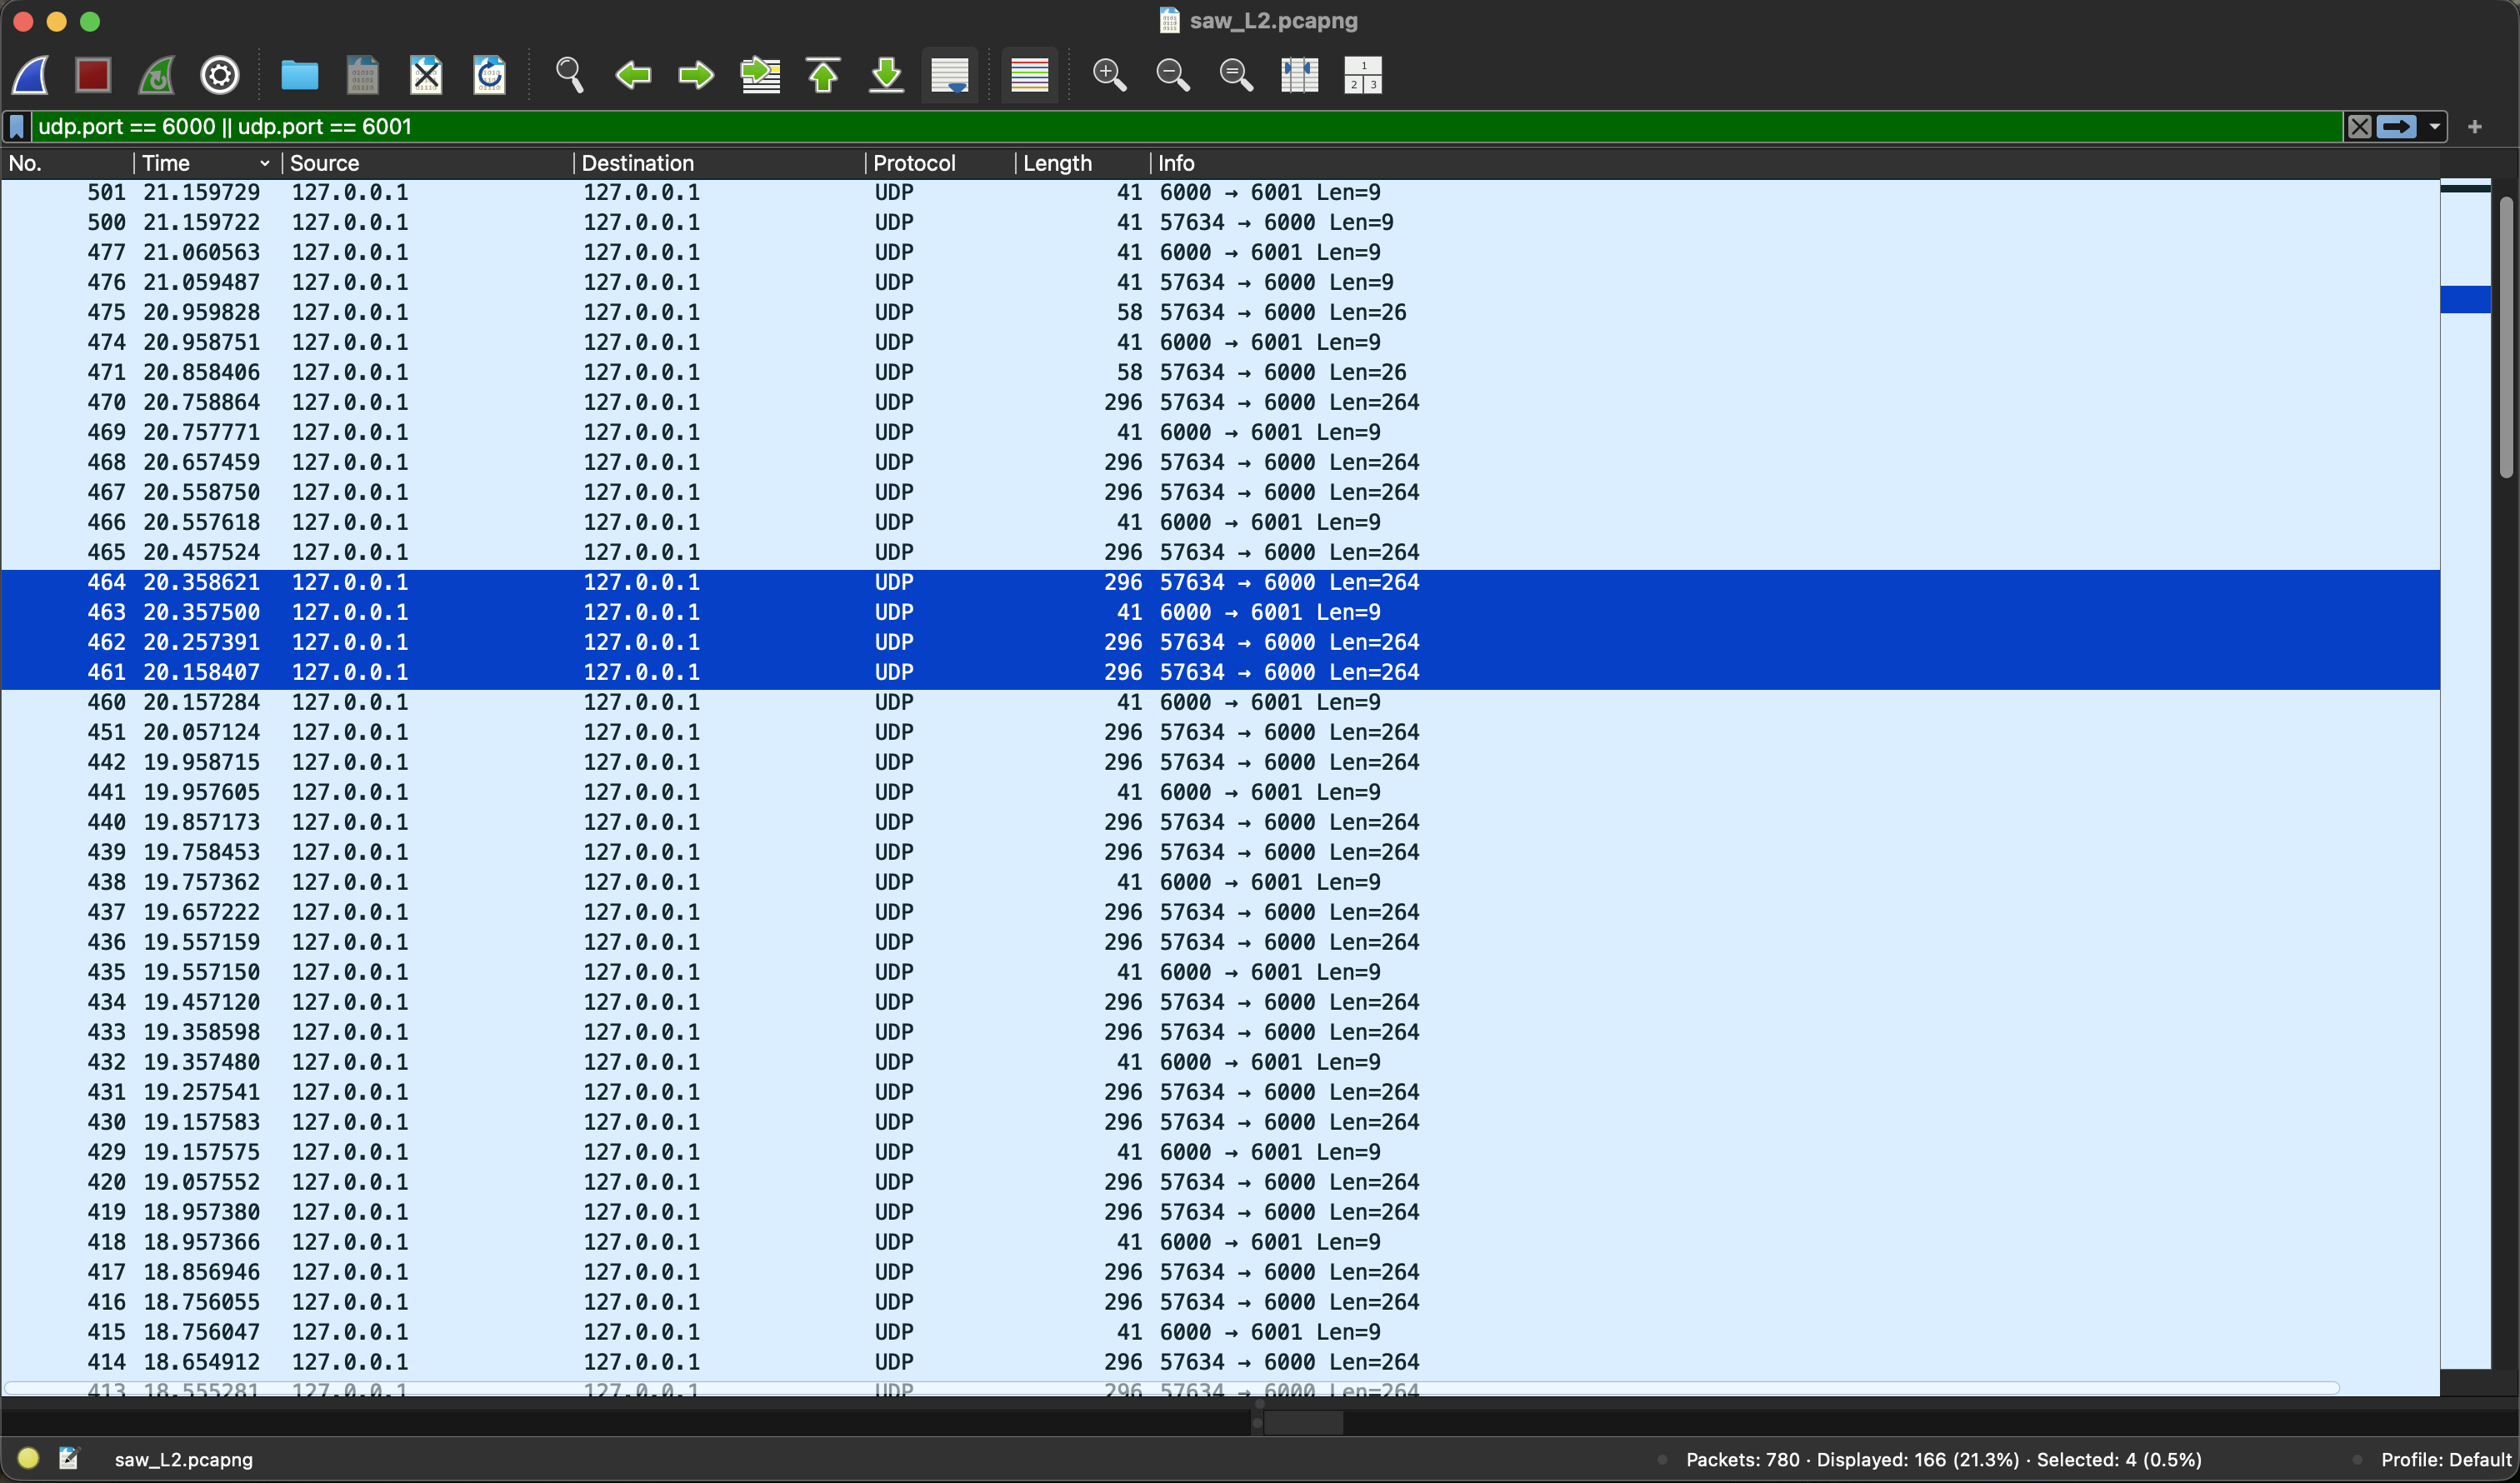
\includegraphics[width=1\textwidth]{imagens/saw_L2_wireshark.png}
    \caption{Captura de tela do Wireshark evidenciando o comportamento no cenário de latência L2/L3 (timeouts e duplicatas).}
    \label{fig:saw_wireshark_latencia}
\end{figure}

\subsection{Análise dos Cenários de Perda (P0 a P4)}
Abaixo são dispostos os resultados obtidos sob taxas de perda artificialmente injetadas na rede, sem latência adicional.

\begin{table}[H]
    \centering
    \caption{Resultados experimentais sob perda de pacotes (SAW)}
    \begin{tabularx}{\textwidth}{c*{4}{Y}}
        \toprule
        \textbf{Cenário} & \textbf{Taxa de Perda (\%)} & \textbf{Throughput Medido (KB/s)} & \textbf{Retransmissões} & \textbf{Tempo Total (s)} \\
        \midrule
        P0 & 0\%   & 2166.35 & 0  & 0.006 \\
        P1 & 1\%   & 116.06  & 1  & 0.110 \\
        P2 & 5\%   & 31.14   & 4  & 0.410 \\
        P3 & 10\%  & 13.88   & 9  & 0.920 \\
        P4 & 25\%  & 5.84    & 21 & 2.136 \\
        \bottomrule
    \end{tabularx}
    \label{tab:saw_perda}
\end{table}

\noindent \textbf{Relação entre perda de pacotes e vazão}:
\\
A análise experimental demonstra que o protocolo Stop-and-Wait é extremamente sensível a perdas de pacotes. A degradação do throughput é severa e não-linear:
\begin{itemize}
    \item \textbf{Cenário P0 (0\% de perda)}: Transmissão limpa. Nenhum pacote é perdido e a vazão atinge o pico de $2166,35\text{ KB/s}$, levando apenas $6\text{ ms}$.
    \item \textbf{Cenário P1 (1\% de perda)}: Ocorre a perda de apenas 1 pacote. O transmissor é obrigado a esperar o estouro completo do timeout de $100\text{ ms}$ antes de retransmitir. Esse único evento eleva o tempo total de $6\text{ ms}$ para $110\text{ ms}$, derrubando a vazão para $116,06\text{ KB/s}$ (uma redução de 94\% em relação à baseline).
    \item \textbf{Cenário P2 (5\% de perda)}: Com 4 retransmissões registradas, o tempo total sobe para $410\text{ ms}$ e a vazão cai para $31,14\text{ KB/s}$.
    \item \textbf{Cenário P3 (10\% de perda)}: Registram-se 9 retransmissões. O tempo total atinge $920\text{ ms}$ e a vazão recua para $13,88\text{ KB/s}$.
    \item \textbf{Cenário P4 (25\% de perda)}: Um quarto dos pacotes (dados ou ACKs) é descartado pela rede. Ocorreram 21 retransmissões, totalizando $2,136\text{ s}$ de tempo decorrido e reduzindo a vazão para apenas $5,84\text{ KB/s}$.
\end{itemize}
Na teoria de protocolos ARQ, a vazão média sob uma probabilidade de perda $p$ em Stop-and-Wait é proporcional a $\frac{1}{1 + p \cdot (TIMEOUT / RTT)}$. Como o $RTT$ real de loopback é inferior a $1\text{ ms}$ e o $TIMEOUT$ é de $100\text{ ms}$, a razão $TIMEOUT/RTT$ é superior a 100. Isso significa que mesmo uma pequena perda de pacote $p$ de $1\%$ tem um impacto amplificado de centenas de vezes no tempo de espera ociosa (\textit{idle time}), mantendo o canal ocioso a maior parte do tempo e destruindo a eficiência da transmissão. Isso ressalta a ineficiência do Stop-and-Wait sob canais com perda.

\subsection{Análise e Comportamento do CRC32}
O cabeçalho do SRTP conta com um campo CRC32 de 32 bits, calculado sobre a concatenação do cabeçalho (com o próprio campo CRC zerado) e do payload de dados.

\noindent \textbf{Descarte silencioso}:
\\
Para garantir a integridade dos dados, o receptor calcula o checksum CRC32 dos pacotes recebidos. Caso ocorra alguma corrupção de bit durante o trânsito (no cabeçalho ou no payload), o CRC32 calculado não baterá com o valor gravado no cabeçalho do pacote, e o método \texttt{parse\_packet} retornará \texttt{None}.
Nesse cenário, o receptor realiza um \textbf{descarte silencioso} (\textit{silent discard}) do pacote, sem enviar qualquer tipo de mensagem de controle de erro (como um NACK) de volta ao transmissor. A razão para essa abordagem é simples: se o CRC32 falhou, significa que a integridade do pacote inteiro está comprometida. Campos cruciais do cabeçalho como o número de sequência (SEQ), a porta ou as flags podem ter sido alterados, tornando impossível para o receptor construir uma resposta coerente ou direcionada ao pacote original. O descarte silencioso delega ao transmissor a responsabilidade de detectar a perda (via estouro do timeout de 100 ms) e realizar a retransmissão de forma segura.

Caso o campo CRC32 não estivesse presente no protocolo, o receptor aceitaria dados corrompidos como válidos e os escreveria no arquivo final, corrompendo a entrega. Além disso, se os bits corrompidos estivessem no cabeçalho (como no número de sequência ou de comprimento do payload), o receptor poderia interpretar erroneamente a ordenação dos blocos ou escrever comprimentos incorretos de dados, dessincronizando o estado de controle de fluxo de ambos os lados e inviabilizando a confiabilidade da sessão.

\begin{figure}[H]
    \centering
    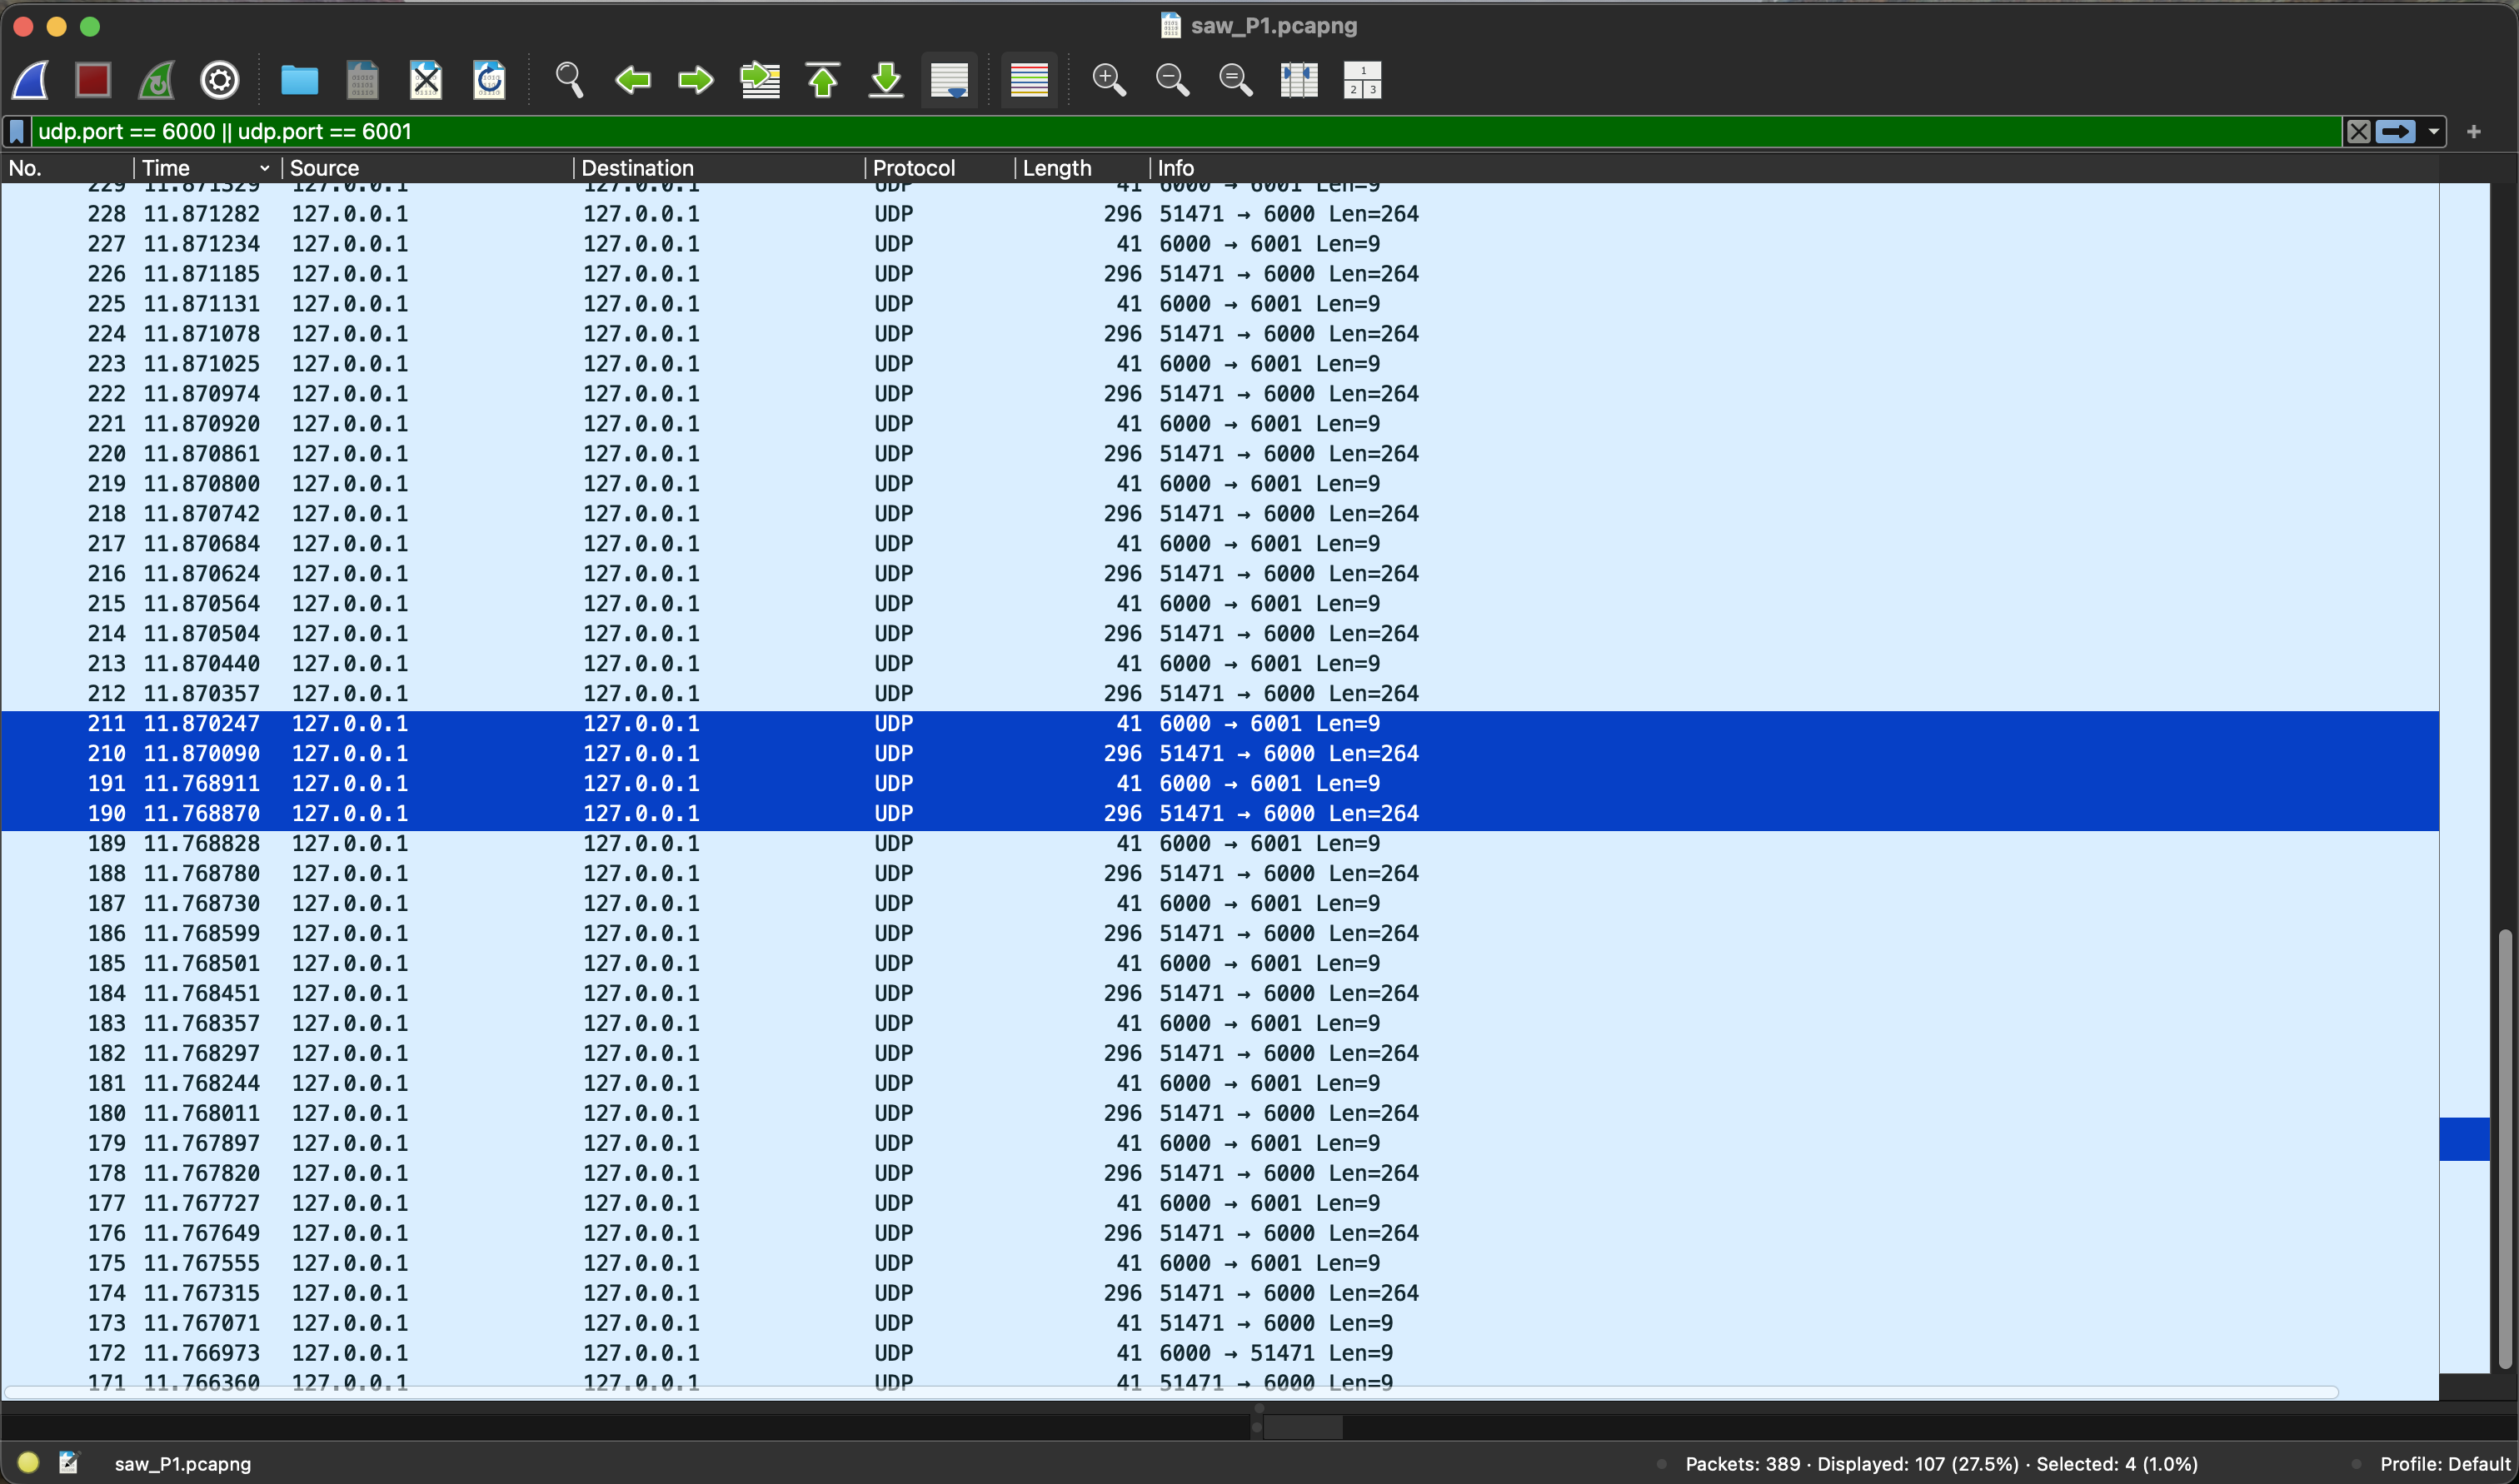
\includegraphics[width=1\textwidth]{imagens/saw_crc_wireshark.png}
    \caption{Evidência de detecção de erro por CRC32 no Wireshark e descarte silencioso.}
    \label{fig:saw_wireshark_latencia}
\end{figure}

\newpage

% ================= SEÇÃO 3: PARTE 2 - GBN E SR =================
\section{Parte 2 — Janela Deslizante (GBN e SR)}

Nesta etapa, implementou-se o controle de fluxo por janela deslizante (\textit{Sliding Window}) utilizando as abordagens Go-Back-N (GBN) e Selective Repeat (SR). A negociação do tamanho da janela ($W$) ocorre de forma dinâmica durante o handshake.

\subsection{Análise Comparativa sob Latência (L0 a L3)}
A tabela abaixo compara o throughput medido dos três protocolos sob as diferentes faixas de latência.

\begin{table}[H]
    \centering
    \caption{Comparação de Throughput (KB/s) sob Latência}
    \begin{tabularx}{\textwidth}{c*{4}{Y}}
        \toprule
        \textbf{Cenário} & \textbf{Stop-and-Wait (SAW)} & \textbf{Go-Back-N ($W=4$)} & \textbf{Go-Back-N ($W=16$)} & \textbf{Selective Repeat ($W=16$)} \\
        \midrule
        L0 & & & & \\
        L1 & & & & \\
        L2 & & & & \\
        L3 & & & & \\
        \bottomrule
    \end{tabularx}
    \label{tab:comparativo_latencia}
\end{table}

\noindent \textbf{Discussão}:
\\
\textit{[Explique como as janelas de transmissão de tamanho maior amortecem o impacto do RTT. Por que o GBN e o SR obtêm um desempenho muito superior ao SAW quando o RTT é alto? Como a taxa máxima teórica de janela deslizante ($W \times L / RTT$) se comporta aqui?]}.

\subsection{Análise Comparativa sob Perda (P1 a P4)}
A perda de pacotes impacta de formas muito distintas o GBN (onde uma perda força a retransmissão em lote de toda a janela a partir do pacote perdido) e o SR (onde apenas o pacote perdido é retransmitido).

\begin{table}[H]
    \centering
    \caption{Custo de Retransmissões: GBN vs SR sob Perdas}
    \begin{tabularx}{\textwidth}{c*{4}{Y}}
        \toprule
        \textbf{Cenário} & \textbf{Go-Back-N ($W=4$)} & \textbf{Go-Back-N ($W=16$)} & \textbf{Selective Repeat ($W=4$)} & \textbf{Selective Repeat ($W=16$)} \\
        \midrule
        P1 & & & & \\
        P2 & & & & \\
        P3 & & & & \\
        P4 & & & & \\
        \bottomrule
    \end{tabularx}
    \label{tab:comparativo_perdas}
\end{table}

\noindent \textbf{Discussão}:
\\
\textit{[Discuta o custo de retransmissão de cada protocolo. Por que a combinação de janela grande com o protocolo GBN em canais de perda (ex: P4) pode ser ineficiente em comparação ao Selective Repeat? Explique detalhadamente com base nos seus dados experimentalmente coletados]}.

\subsection{Análise Comparativa sob Reordenação (R0 a R2)}
\textit{Este é o ponto central da avaliação da Parte 2.} Sob reordenação, os pacotes chegam fora de ordem ao destinatário.

\noindent \textbf{Comportamento do Go-Back-N (GBN)}:
\\
\textit{[Descreva o comportamento do GBN quando recebe um pacote fora de ordem. Dica: ele descarta o pacote e envia um NACK pedindo o SEQ esperado. O transmissor é forçado a voltar e reenviar toda a janela. Mostre esse descarte e retransmissão em lote nas capturas do Wireshark].}

\noindent \textbf{Comportamento do Selective Repeat (SR)}:
\\
\textit{[Descreva a bufferização fora de ordem do SR. Dica: o receiver aceita os pacotes contidos na janela ativa, guarda-os temporariamente no buffer, envia ACKs individuais e, quando o pacote ausente chega, faz o \textit{flush} para a aplicação entregando na ordem correta. Mostre esse fluxo de bufferização e entrega tardia nas suas capturas].}

\begin{figure}[H]
    \centering
    % \includegraphics[width=0.9\textwidth]{capturas/gbn_reorder_wireshark.png}
    \caption{Captura de tela demonstrando o descarte e retransmissão em lote do GBN sob reordenação.}
    \label{fig:gbn_reorder}
\end{figure}

\begin{figure}[H]
    \centering
    % \includegraphics[width=0.9\textwidth]{capturas/sr_reorder_wireshark.png}
    \caption{Captura de tela demonstrando a bufferização fora de ordem e entrega ordenada no SR.}
    \label{fig:sr_reorder}
\end{figure}

\subsection{Impacto do Tamanho de Janela ($W=4$ vs. $W=16$)}
\textit{[Compare o comportamento de utilizar janelas pequenas ($W=4$) versus janelas maiores ($W=16$). Aborde o trade-off entre o potencial de throughput de uma janela larga contra o desperdício de banda devido a retransmissões massivas no GBN sob altas perdas.]}

\newpage

% ================= SEÇÃO 4 =================
\section{Conclusão}
\textit{[Resuma as principais observações obtidas através dos testes. Fundamentado nos dados empíricos apresentados neste relatório, explique em qual tipo de canal/ambiente cada protocolo (SAW, GBN, SR) é mais apropriado e justifique o porquê (por exemplo, SAW para redes muito simples com baixo RTT e sem perda, GBN para canais de alta latência e baixa perda devido à simplicidade do receptor, SR para redes com latência e perdas/reordenações severas).]}
\newpage

% ================= REFERÊNCIAS =================
\section*{Referências}
\addcontentsline{toc}{section}{Referências}

\begin{enumerate}
  \item INEP. \textbf{Microdados do Censo Escolar da Educação Básica 2023}. Disponível em: \url{https://www.gov.br/inep/pt-br/acesso-a-informacao/dados-abertos/microdados/censo-escolar}. Acesso em: jun. 2026.
  \item INEP. \textbf{Resultados do IDEB 2023}. Disponível em: \url{https://www.gov.br/inep/pt-br/areas-de-atuacao/pesquisas-estatisticas-e-indicadores/ideb/resultados}. Acesso em: jun. 2026.
  \item PNUD; IPEA; FJP. \textbf{Atlas do Desenvolvimento Humano no Brasil}. Disponível em: \url{https://basedosdados.org/dataset/br-pnud-idhm}. Acesso em: jun. 2026.
  \item MICROSOFT. \textbf{Documentação do Azure Synapse Analytics}. Disponível em: \url{https://learn.microsoft.com/pt-br/azure/synapse-analytics/}. Acesso em: jun. 2026.
\end{enumerate}

\end{document}